%%%%%%%%%%%%%%%%%%%%%%%%%%%%%%%%%%%%%%%%%%%%%%%%%%%%%%%%%%%%
%%% LIVECOMS ARTICLE TEMPLATE FOR BEST PRACTICES GUIDE
%%% ADAPTED FROM ELIFE ARTICLE TEMPLATE (8/10/2017)
%%%%%%%%%%%%%%%%%%%%%%%%%%%%%%%%%%%%%%%%%%%%%%%%%%%%%%%%%%%%
%%% PREAMBLE
\documentclass[9pt,bestpractices]{molsim}
% Use the 'onehalfspacing' option for 1.5 line spacing
% Use the 'doublespacing' option for 2.0 line spacing
% Use the 'lineno' option for adding line numbers.
% The 'bestpractices' option for indicates that this is a best practices guide.
% Omit the bestpractices option to remove the marking as a LiveCoMS paper.
% Please note that these options may affect formatting.

\usepackage{lipsum} % Required to insert dummy text
\usepackage[version=4]{mhchem}
\usepackage{siunitx}
\DeclareSIUnit\Molar{M}
\newcommand{\versionnumber}{1.3}  % you should update the minor version number in preprints and major version number of submissions.
\newcommand{\githubrepository}{\url{https://github.com/myaccount/homegithubrepository}}  %this should be the main github repository for this article
\graphicspath{{figures/}}
%%%%%%%%%%%%%%%%%%%%%%%%%%%%%%%%%%%%%%%%%%%%%%%%%%%%%%%%%%%%
%%% ARTICLE SETUP
%%%%%%%%%%%%%%%%%%%%%%%%%%%%%%%%%%%%%%%%%%%%%%%%%%%%%%%%%%%%
\title{Physical quantities in molecular simulation}

\author[1*]{David A. Kofke}
\affil[1]{University at Buffalo}

\corr{kofke@buffalo.edu}{DAK}  % Correspondence emails.  FMS and FS are the appropriate authors initials.


\begin{document}

\maketitle

In this chapter we review the types of physical quantities encountered
in a molecular simulation.

\section{Several types of quantities are of interest}
\subsection{State variables}\label{state-variables}

Molecular simulation describes physical systems, particularly ones that
are usually examined in the context of chemical thermodynamics.
Naturally, the quantities encountered in thermodynamics are relevant to
molecular simulation. This includes the temperature and internal energy,
pressure and volume, and moles and chemical potential; additional
thermodynamic state variables arise in mixtures, and other cases such as
when surface tension is relevant.

It is important to pay attention to the pairing of the variables as just
given. Here they are again:
\begin{table}[h]
  \centering
  \caption*{}
  \label{my-label}
  \begin{tabular}{ll}
    \hline
  \hline
  \multicolumn{1}{c}{\textbf{Extensive Variable}} & \multicolumn{1}{c}{\textbf{Conjugate Field}} \\ \hline
  Internal energy, $E$                            & Temperature, $T$                             \\
  Volume, $V$                                     & Pressure, $P$                                \\
  Number of molecules, $N$                        & Chemical potential, $\mu$                    \\ \hline
  \end{tabular}
  \end{table}

Note that each pair comprises an extensive variable, one that scales
linearly with the system size, and a conjugate field variable, which is
intensive and thus size-independent. The full specification of the
thermodynamic state requires that one of each pair be specified. The
value of the each of the resulting dependent variables is then given as
some sort of an average over all the microscopic configurations of the
molecules of the system. One of the aims of molecular simulation is to
perform this averaging and report, for example, how the internal energy
depends on temperature, pressure and number of molecules for a system of
interest.

Different molecular simulation algorithms are required for different
choices of the dependent and independent state variables.
Independent variables are those which can be used to specify the thermodynamic state of the system; that is, simulations are conducted in a particular ensemble with a particular choice of values for specified independent variables.
Common choices
for the independent variables are \emph{EVN} (the microcanonical ensemble), \emph{TVN}
(canonical ensemble), \emph{TPN} (isothermal-isobaric ensemble) and \emph{TV$\mu$}
(grand-canonical ensemble).
For example, simulations specifying \emph{EVN} hold temperature, volume and number of particles constant.
Other choices for independent variables are possible, but note that
there must always be at least one extensive variable in the set;
otherwise there is nothing to specify the absolute size of the system,
and the state is not well defined (violation of the Gibbs phase rule).

\subsection{Configuration variables}\label{configuration-variables}

Molecular simulation of course deals with the arrangements and
rearrangements of molecules, so variables specifying the molecular
configurations play a central role. The ``configuration'' is given by
all those variables needed to fully specify the microscopic state of the
set of molecules and their atoms. This includes primarily the positions
and momenta of all atoms. We use the symbol \textbf{r} to represent the
position vector, and \textbf{p} the momentum vector. In Cartesian
coordinates, the momentum is simply related to the velocity \textbf{v}
through \textbf{p} = m\textbf{v}, where m is the mass. Molecular
position and momentum vectors are sometimes used, and these normally
apply to the center of mass of the molecule. Orientation variables
(position and momentum) may arise naturally in the treatment of
molecules. Sometimes it is more convenient to specify the configuration
in terms of molecular position and momentum, with atomic coordinates
given in a molecule-based frame, such that atom positions are specified
in terms of bond angles and bond distances. We will postpone discussion
of these complicating features until later, when we examine more complex
and realistic molecular models.

If an extensive variable is not included in the state variables as
discussed above, it becomes a configuration variable and is part of the specification of the microscopic state of the system.
So in an isobaric
simulation (in which pressure is imposed instead of the volume), the
volume will fluctuate as part of the simulation process, and the full
microscopic state has the instantaneous volume as one if its variables.
Likewise, in the grand-canonical ensemble, the number of molecules is a
fluctuating configuration variable. Configuration variables of this type
are averaged over many configurations to yield the corresponding
thermodynamic state variable (\emph{e.g.}, in isothermal systems the
thermodynamic energy is an average of configurational energy).

Special mention should be made of time, which plays a central role in
molecular dynamics but normally has no significance in Monte Carlo
simulations.

Note that this discussion applies to systems modeled
classically (i.e., using classical mechanics). Electronic degrees of freedom
are of interest in some cases (e.g., chemical reactions), and these may be
treated with quantum mechanics. For light atoms and/or low temperatures,
quantum effects are relevant also to the atomic nuclei, and special measures
must be applied in these cases.

\subsection{Physical properties}\label{properties}

Other important physical quantities can be computed given a specific
molecular configuration. In addition to the energy, forces are needed to advance a molecular dynamics simulation.
The virial is routinely computed to measure the pressure, and the stress
tensor may be needed to evaluate rheological properties. Indeed, it can
be quite enlightening to learn and implement the formulas used to
compute common but nontrivial physical properties (\emph{e.g.},
diffusivity, viscosity, dielectric constant) from quantities that are
averaged over molecular configurations. Other properties of interest
characterize uniquely molecular behaviors. An example is the radial
distribution function, which quantifies the molecular structure.

All of the foregoing properties are special in that they have
``instantaneous'' values that can be associated with each configuration.
This can be contrasted with the ``statistical'' properties, such as the
entropy and free energy. These properties do not have values
defined for an individual configuration. Instead these properties depend
on features of the entire ensemble of configurations. For example, the
entropy is related to the number of distinct configurations that can be
formed consistent with particular values of $E$, $V$, and $N$. Hence there is
no ``entropy of a configuration'', but there is an entropy of an
ensemble of configurations.
Thus these statistical properties can \emph{only} be calculated from an ensemble of configurations.

\subsection{Model parameters}\label{model-parameters}

Another class of physical quantities arises with the specification of
the molecular model. Classical models of molecular interactions are
defined in terms of simple functions. These functions take as inputs the
atomic distances and from them output a potential energy, so at a
minimum (with some exceptions) they introduce a characteristic length
and a characteristic energy in their definition. As an aside we note
that the ``size'' (and, more obviously, the ``energy'') of a model
molecule is not a well defined quantity, and that it is only through
interaction with another molecule that the ``size'' manifests itself.
Consequently the characteristic size and energy are more properly
associated with the pair interaction rather than with the molecule
itself.

More complex model potentials usually introduce more than one size and
energy parameter. These may introduce force constants for vibrations,
bends, and torsional motions, bond lengths, asymmetric potential
parameters, and so on. These models also may be constructed in part
using Coulombic point charges or point multipoles.

\section{Dimensions, Units, and
Scaling}\label{dimensions-units-and-scaling}

The table below shows typical values of commonly used
molecular variables. Because simulations involve on the order
10\textsuperscript{3} molecules instead of 10\textsuperscript{23},
values for the mass, energy, and volume are very small numbers when
expressed in the common macroscopic units (meters, Joules, grams,
\emph{etc}). Working with such small numbers can be inconvenient, but
the remedy is obvious and simple: use different units, ones more
appropriate to molecular-scale magnitudes. Thus we can work with
Angstroms, Daltons, ergs, and so on. An alternative approach is to work
with dimensionless variables, in which all physical properties are
scaled using appropriate combinations of a characteristic size, energy
and/or mass (these three are sufficient to de-dimensionalize most
properties that arise in molecular simulation); these values usually
come from an appropriate atomic mass and parameters of a model for the
pair potential. There are two advantages to working with dimensionless
groups. First, their use ensures that all unit conversions are handled
automatically. For example, in isobaric simulations it is necessary to
evaluate the group $PV/k_{\rm B}T$. If dimensionless quantities are used ($P^* =
P\sigma^3/\epsilon$, $V^* = V/\sigma^3$, $T^* = k_{\rm B}T/\epsilon$, where $\epsilon$
and $\sigma$ are a characteristic energy and size, respectively), then the
group is correctly given by $P^*V^*/T^*$. However, if $P$ is given in
bar, $V$ is in cubic Angstroms, and $T$ is in Kelvins, then one must
pay heed to use an appropriate value for Boltzmann's constant to ensure
that the units cancel properly. Such problems arise in many places, and
they make programming tiresome and error-prone. If all physical
quantities are scaled by the same characteristic values these problem
vanish.

\begin{figure}
  \centering
  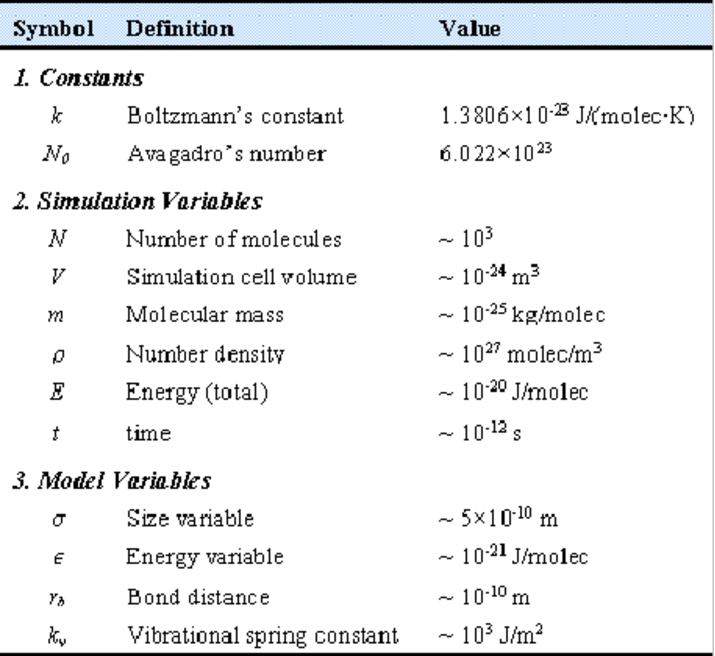
\includegraphics[width=\textwidth]{SimElements_figures/magnitudes.pdf}
  \caption{\label{fig:magnitudes}Typical magnitudes of variables encountered in a molecular simulation.}
\end{figure}


Note that the benefits gained from using dimensionless quantities are
equally well realized if one takes care to use a consistent set of units
within the simulation. Agree that all properties within the simulation
will be expressed in, for example, picoseconds, Angstroms, and Daltons,
and that temperature is always actually $k_{\rm B}T$, \emph{etc.}, and the units
will again take care of themselves. In fact, this is exactly what is
done when one scales by $\sigma$ and $\epsilon$; one is defining a new system of units
in which these parameters are unity. A dimensionless length $L/\sigma = 5$ is
perfectly well described as ``five sigmas'', just as one speaks of $L =
5\AA$ as ``5 Angstroms'' and writes just as well as ``$L/\AA$ = 5''. A
dimensionless pressure $P^* = 3$ (as defined above) is ``three epsilons per
cubic sigma'', although no one speaks of it this way. In this view,
insertion of values for $\sigma$ and $\epsilon$ to recover conventional units is no
different than applying a conversion from (say) Angstroms to recover
meters.

Regardless of the choice of an internal system, the units will not have
a desired or familiar form for every property, in which case a
conversion can be performed upon input or output to express the property
in a preferred unit. It is a good idea to keep this conversion process
isolated to the input/output segments of the program, and to work with a
self-consistent units at all other places. One exception to this rule
arises. It can be computationally expedient to work with a coordinate
system that ranges over a unit length, so that all atom coordinates lie
between 0 and 1 (or, alternatively, $-1/2$ and $+1/2$). Then special care
must be taken to rescale distances and velocities so that the values are
consistent with the simulation units. We discuss this choice further in
the section on periodic boundary conditions.

For very simple systems, molecular modelers often prefer to keep the
simulation inputs and outputs in scaled form. This merely postpones the
conversion to more traditional units. This might be done because when
the simulation is performed there are no physical values for $\sigma$ and $\epsilon$ in
mind (no real physical system is being modeled). Sometimes there is no
intention of ever converting the values to ``real'' units, because one
is interested only in qualitative behaviors of the model, or in
comparing the simulation to predictions from a statistical mechanical
theory applied to the same model.

As is likely apparent by now, unit handling can be complex and is a frequent source of error.
In general, regardless of what approach is chosen, we recommend that user-facing components of programs use programming libraries which accommodate and handle units so that users can provide or obtain values in the units they prefer and still have the intended outcome.
For example, a user might choose to provide a pressure in atmospheres or Pascals; ideally, both users should be able to obtain correct results without having to know what units your program will prefer.
Several Python libraries (such as \texttt{pint} and \texttt{simtk.util} and probably others) are available which facilitate this process, and reduce the potential for critical errors due to unit handling in input or output.

Perhaps it is worthwhile to consider an example demonstrating conversion
to and from scaled units. The Lennard-Jones (LJ) equation of state (which describes how
the pressure depends on temperature and density for the LJ model fluid)
is very well known from molecular simulation studies (ref). One can find
extensive data and accurate empirical models in the literature. All of
these data are presented in sigma-epsilon units (\emph{i.e.}, units in
which the LJ size and energy parameters are 1). Further, it is not
unusual to find works in which the LJ equation of state is compared to
experimental data for a real system. The aim of these studies is to find
values (expressed in real units) of the LJ parameters such that the LJ
model data coincides with the experimental data as much as possible.
Thus one might arrive for example at the values of $\sigma = 3.790\AA$ and $\epsilon/k_{\rm B} =
142.1$ K as ``best'' values for methane. With
these values in hand, one can go on to estimate the pressure of methane
at 0.0183 mol/cm\textsuperscript{3} and 167 K. The first step is to put
these values in dimensionless form using the methane LJ parameters

$\rho^* \equiv \rho\sigma^3 = (0.0183~{\rm mol/cm}^3)(3.790 \times
10^{-8} {\rm cm})^3(6.022 \times 10^{23} \frac{{\rm molecules}}{{\rm mole}}) = 0.6$

$T^* = T/(\epsilon/k_{\rm B}) = (167~{\rm K})/(142.1~{\rm K}) = 1.174$

The LJ model at these state conditions has a dimensionless pressure $P^* =
0.146$. For the methane $\sigma$ and $\epsilon$ values, this corresponds to a ``real''
pressure of

$P = 0.146 (142.1~{\rm K})(13.8~{\rm MPa}\cdot\AA^{3}/{\rm molecule})/(3.790\AA)^{3} = 5.3~{\rm MPa}$

or 53 bars.

\subsection{Peculiarities of the hard sphere model with respect to units}

Let us finish this chapter by highlighting a peculiar feature of the
hard-sphere model. In the HS model the potential is infinite for atoms
separated by less than one diameter $\sigma$, and is zero otherwise.

\begin{figure}
  \centering
  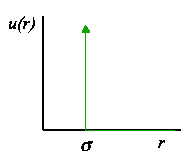
\includegraphics[width=5 cm]{SimElements_figures/image001}
  \caption{\label{fig:HS} The hard-sphere potential.}
\end{figure}

The HS diameter introduces a natural length scale for the model.
However, the model defines \emph{no natural energy scale}, inasmuch as
zero and infinity are not suitable characteristic values. In fact, in
hard-sphere systems the temperature provides the only suitable scale for
the energy. Consequently, the value of dimensionless groups (such as
$P\sigma^3/k_{\rm B}T$) cannot depend on the temperature; the only
independent, dimensionless state variable that can be constructed is the
density $\rho\sigma^3$. The hard-sphere model has important
simplifying features such as this, and yet it captures an essential
feature (harsh repulsion at short distances) of the behavior of real
atoms. This is a good balance of simplicity and realism, and thus the
hard-sphere model---examined through the application of theory and
molecular simulation---has played a very important role in the
development of our understanding of real fluids and solids.


%\section{Author Contributions}
%\section{Other Contributions}

\end{document}
